%++++++++++++++++++++++++++++++++++++++++
% Don't modify this section unless you know what you're doing!
\documentclass[letterpaper,12pt]{article}
\usepackage{tabularx} % extra features for tabular environment
\usepackage{amsmath}  % improve math presentation
\usepackage{amssymb}
\usepackage{graphicx} % takes care of graphic including machinery
\usepackage[margin=1in,letterpaper]{geometry} % decreases margins
\usepackage{cite} % takes care of citations
\usepackage[final]{hyperref} % adds hyper links inside the generated pdf file
\usepackage{float}
\usepackage[toc,page]{appendix}
\usepackage{listings}
\usepackage{siunitx}
\usepackage{pdfpages}
\usepackage{fancyhdr}
\usepackage{caption}
\usepackage{booktabs}


\setlength{\parskip}{1em}
\setlength\parindent{0pt}


\hypersetup{
	colorlinks=true,       % false: boxed links; true: colored links
	linkcolor=blue,        % color of internal links
	citecolor=blue,        % color of links to bibliography
	filecolor=magenta,     % color of file links
	urlcolor=blue
}


\newcommand{\degrees}{^\circ}
\newcommand{\di}{\partial}
%++++++++++++++++++++++++++++++++++++++++

\title{Title}
\author{}
\date{\today}											% Date

\makeatletter
\let\thetitle\@title
\let\theauthor\@author
\let\thedate\@date
\makeatother

\pagestyle{fancy}
\fancyhf{}
\rhead{\theauthor}
\lhead{\thetitle}
\cfoot{\thepage}


\begin{document}

\begin{titlepage}
	\centering
    \vspace*{-1 cm}
    
\includegraphics[scale = 0.5]{UW.jpg}\\	% University Logo
    \textsc{\Large Department of Mechanical and Mechatronics Engineering}\\[2.0 cm]
	\rule{\linewidth}{0.2 mm} \\[0.4 cm]
	{ \huge \bfseries \thetitle}\\
	\rule{\linewidth}{0.2 mm} \\[1.5 cm]

	\begin{minipage}[t]{0.4\textwidth}
		\begin{flushleft} \large
			\emph{Author:}\\
            James Graham-Hu \\
			\end{flushleft}
			\end{minipage}~
			\begin{minipage}[t]{0.4\textwidth}
			\begin{flushright} \large
			\emph{Student Number:} \\
				20555690 \\
		\end{flushright}
	\end{minipage}\\[2 cm]
	Date:
	{\large \thedate}\\[2 cm]
	\vfill

\end{titlepage}
%%%%%%%%%%%%%%%%%%%%%%%%%%%%%%%%%%%%%%%%%%%%%%%%%%%%%%%%%%%%%%%%%%%%%%%%%%%%%%%%%%%%%%%%%
\pagenumbering{gobble}
\thispagestyle{empty}
%%letter of submittal
\thedate\\

William Melek, Director\\
Mechatronics Engineering\\
University of Waterloo\\
Waterloo, Ontario\\
N2L 3G1\\

Dear Professor Melek,\\

This report entitled "Title", was prepared as my Work Report 400 for the Department of Mechanical and Mechatronics Engineering at the University of Waterloo for the 4A term. Purpose of report.\\

Description of Amii.\\

Description of project and motivation behind project.\\


Thank yous.
This report was written entirely by  me and has not received any previous academic credit at this or any other institution.\\

Sincerely,\\

James Graham-Hu\\
ID 20555690\\
4A Mechatronics Engineering



\pagebreak
%%%%%%%%%%%%%%%%%%%%%%%%%%%%%%%%%%%%%%%%%%%%%%%%%%%%%%%%%%%%%%%%%%%%%%%%%%%%%%%%%%%%%%%%%
\pagenumbering{roman}
\tableofcontents
% \setcounter{page}{1}
\pagebreak
\listoffigures
\pagebreak
\listoftables
\pagebreak


%%%%%%%%%%%%%%%%%%%%%%%%%%%%%%%%%%%%%%%%%%%%%%%%%%%%%%%%%%%%%%%%%%%%%%%%%%%%%%%%%%%%%%%%%
\pagenumbering{arabic}
\section{Summary}
Summary
\pagebreak
\section{Introduction}
\subsection{Problem Definition}
Demos can provide an interesting and intuitive way to demonstrate the capabilities and advantages of machine learning to interested parties. Although a few software demos exist at Amii, there is currently no demo that implements machine learning on a hardware system. The advantage of implementing machine learning on hardware is that it is a hands-on way of demonstrating how machine learning can improve a system or be applied to a problem. The problem this project addresses is the lack of a hardware demo to demonstrate machine learning at Amii.

\subsection{Objective}
The automatic levelling wrist, developed by Dylan A. J. Brenneis as part of his Master's thesis in 2019, \cite{d.j.a.brenneis} is a good candidate for a hardware system that can be improved with machine learning. The objective of this project is to use machine learning to improve the automatic levelling wrist in a meaningful and  demonstrable way.


\section{Background}
\subsection{Automatic Levelling Wrist Background}
Powered wrist movement is rare in commercial systems, and many powered protheses have only one degree of freedom (DOF), usually rotation \cite{n.m.bajaj}. These limitations in ease of wrist movement in many upper limb prostheses force people with major upper limb loss to use compensatory movements \cite{s.l.carey}. Compensation occurs with trunk, shoulder, and elbow movements, and has been associated with causing musculoskeletal pain in the neck, upper back, shoulder, and remaining arm \cite{k.ostlie}.

A two DOF automatic levelling wrist was developed by Dylan J. A. Brenneis in 2019 that addresses the issues with ease of wrist movement in wrist prosthetics \cite{d.j.a.brenneis}. The two DOF automatic levelling wrist provides two degrees of freedom, rotation and flexion of the wrist. The user has the ability to switch between controlling the position of the flexion, or letting it automatically level itself to maintain its angle with the ground (see figure \ref{fig:auto_levelling}). The rotation of the wrist is always automatically leveled to be flat with the ground. These features are shown to reduce compensatory movements in vertically-oriented tasks. However, the current implementation of the automatic levelling wrist is reported as unreliable and unintuitive in user tests \cite{d.j.a.brenneis}. Possible reasons for a feeling of unreliability from users could be a result of slow response time, oscillations, and poor disturbance rejection in the automatic levelling system.

\begin{figure}[H]
\centering 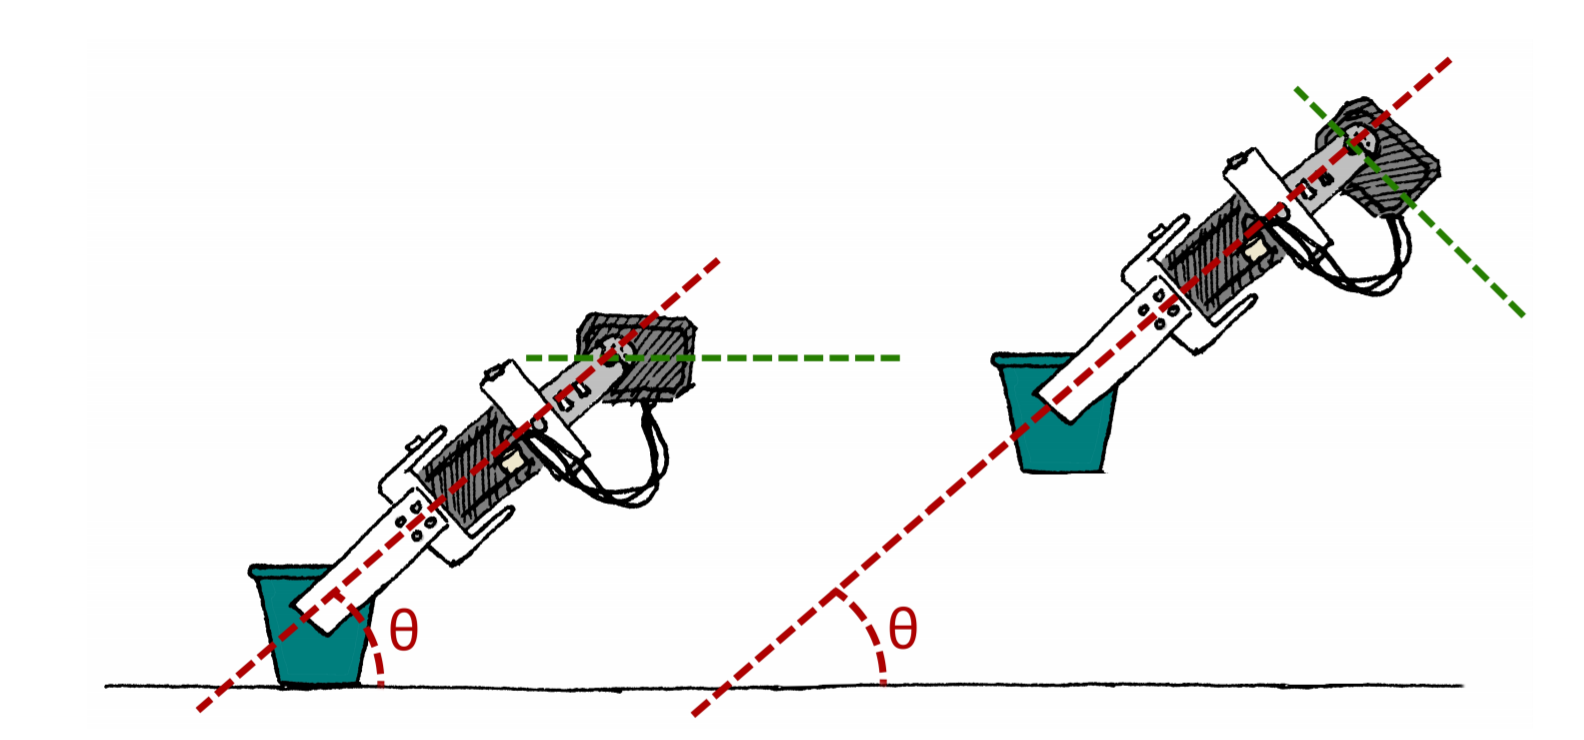
\includegraphics[width=0.8\columnwidth]{auto_levelling.png}
\caption{\label{fig:auto_levelling}Automatic levelling of the flexion. The angle, $\theta$, of the flexion servo is constant with the ground as the arm moves (represented by the green dashed line) \cite{d.j.a.brenneis}.}
\end{figure}

Figure \ref{fig:slw_diagram} shows the design of the automatic levelling wrist. It should be noted that the automatic levelling wrist is designed as a bypass protheses so that an able-bodied person is able to use it. A higher statistical power is able to be achieved in a more time efficient way by running trials with able-bodied persons, because of limitations in participant availability when running trials with participants affected by amputation \cite{d.j.a.brenneis}.

\begin{figure}[H]
\centering 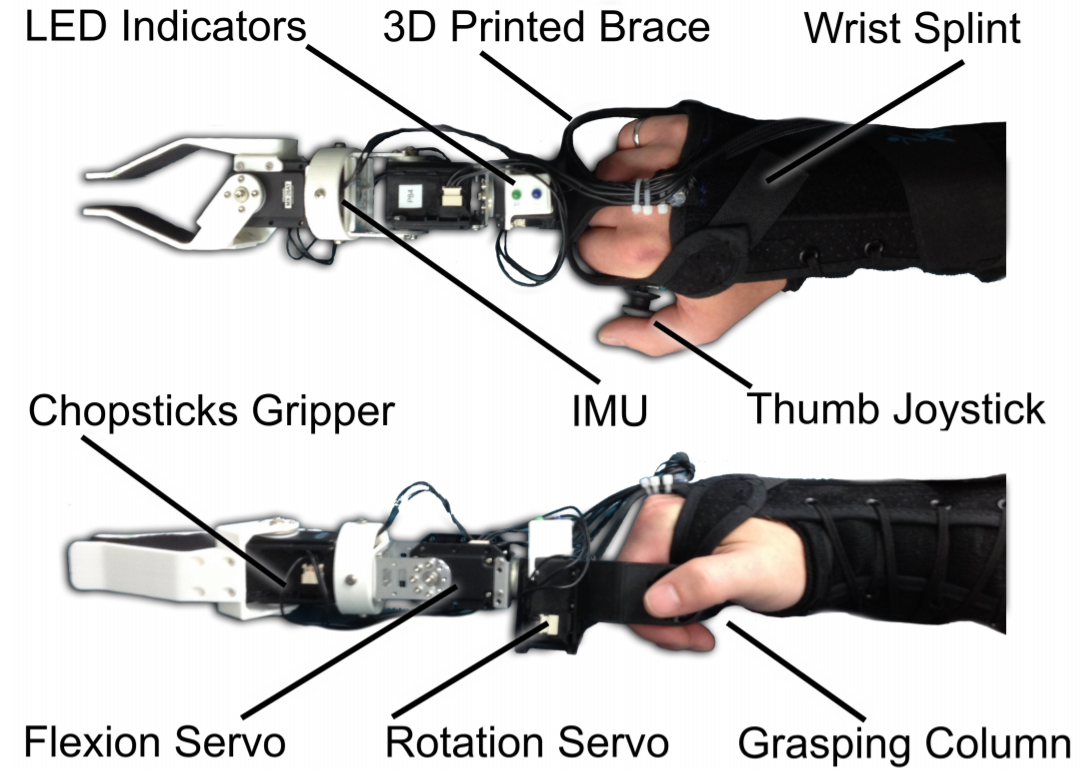
\includegraphics[width=0.8\columnwidth]{slw_diagram.png}
\caption{\label{fig:slw_diagram}Diagram of the automatic levelling wrist bypass protheses \cite{d.j.a.brenneis}.}
\end{figure}

\subsubsection{Automatic Levelling Method}
The wrist is automatically leveled using an Adafruit 9-DOF absolute orientation IMU fusion breakout (BNO055) attached to the base of the gripper, as seen in figure \ref{fig:slw_diagram}, and two independent PID controllers, one for the rotation servo and one for the flexion servo. The gravity vector from the IMU is used to calculate the current angle of rotation and flexion. The error between the calculated angle and the setpoint is fed into the PID controller to generate a control signal for the servo. The setpoint for the rotation servo is always set to $180\degrees$ while the setpoint for the flexion servo is set to where the user last moved it to before switching to automatic levelling. Figure \ref{fig:angles} shows the definitions for the coordinate system, the angle of rotation, $\phi$, and the angle of flexion, $\theta$.

\begin{figure}[H]
\centering 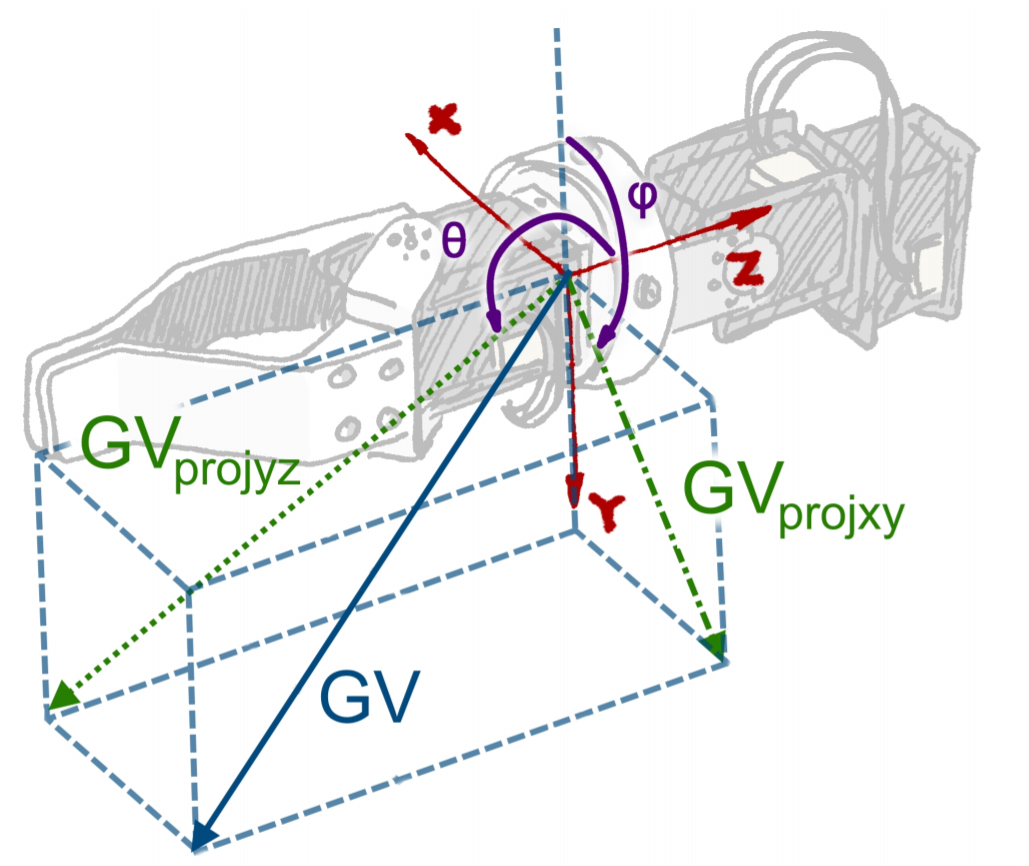
\includegraphics[width=0.8\columnwidth]{angles.png}
\caption{\label{fig:angles}Coordinate system and angles, $\phi$ and $\theta$. The projections of the IMU gravity vector (GV) can be used to calculate $\phi$ and $\theta$ \cite{d.j.a.brenneis}.}
\end{figure}

$\phi$ is defined as the angle between the negative y-axis and the projection of the gravity vector in the x-y plane. $\theta$ is defined as the angle between the positive z-axis and the projection of the gravity vector projected in the y-z plane.

Figure \ref{fig:servo_system} shows the block diagram for one servo in the automatic levelling wrist. A simple PID control loop controls the position of the servo. The equation for the PID controller signal, $u(t)$, is given by equation \ref{eq:pid}. The servo position is summed with a disturbance and fed through the IMU to acquire either $\phi$ or $\theta$. The block diagram for the rotation and flexion servos are the same other than the $K_p$, $K_i$, and $K_d$ gain values for the PID controllers, the IMU function, and the value of the disturbance, $d(t)$. The disturbance is considered as the angle of the user's wrist with respect to a fixed coordinate system that is coincident with the user's wrist when it is completely level with the ground. Note that in the actual implementation of the control loop, the disturbance and servo position aren't directly used. Rather, they are implicitly included when the IMU measures the gravity vector since the gravity vector changes based on the disturbance and servo positions.

\begin{equation}
	\label{eq:pid}
	u(t) = K_p e(t) + K_i \int e(t) dt + K_d \frac{de(t)}{dt}
\end{equation}

\begin{figure}[H]
\centering 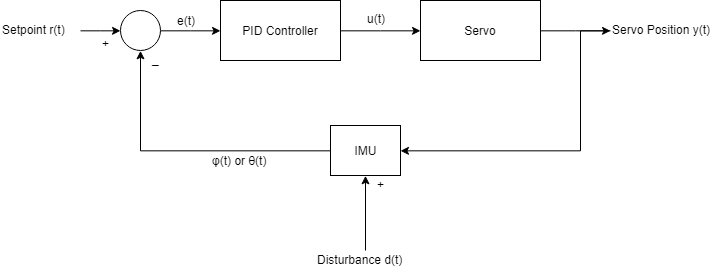
\includegraphics[width=0.8\columnwidth]{servo_system.png}
\caption{\label{fig:servo_system}Block diagram of the control loop for one servo.}
\end{figure}

\subsection{Neural Network Background}
In machine learning, neural networks are used to represent non-linear functions by making use of one or more hidden layers and activation functions. Figure \ref{fig:nn} shows the structure of a neural network with one hidden layer. In this network, the input vector, $X$, is multiplied by the weight matrix $W_{0}$ and summed with the bias vector $b_{0}$. The result of that is then put through an activation function, giving a vector of activations. These activations are then multiplied by the weight matrix $W_{1}$ and summed with the bias vector $b_{1}$ to give the output, $y$. The output can also be put through an activation function. In regression, a linear activation function is mostly used on the output. Activation functions used in the hidden layer include but are not limited to the hyperbolic tangent, sigmoid, and rectified linear unit (ReLU) functions. The choice of activation function is dependent on the application of the neural network.

\subsubsection{Backpropagation}
Learning for a neural network is most commonly accomplished by backpropagation. Backpropagation is performed by calculating the derivative of the squared error of the neural network with respect to each weight in the network. The squared error of the neural network is defined in equation \ref{eq:sq_error}. The equation is divided by two to simplify the derivative. Since the entire network including its activation functions is differentiable, the chain rule can be used to backpropagate the error between the neural network's output and what the output should be (the label) back to the weights. Equation \ref{eq:nn_equation} is the update function used for weight $w_{i,j}$ in the neural network which updates the weights at a learning rate $\alpha$.

\begin{equation}
	\label{eq:sq_error}
	E = \frac{1}{2}(y_{true} - y_{pred})^2
\end{equation}

\begin{equation}
	\label{eq:nn_equation}
	w_{i, j} \leftarrow w_{i,j} + \alpha \frac{\di E}{\di w_{i, j}}
\end{equation}

\subsubsection{Levenberg-Marquardt Algorithm}\label{sec:levenberg}
Another method for training neural networks is using the Levenberg-Marquardt algorithm. The Levebnerg-Marquardt algorithm uses the jacobian of the output with respect to the weights of the neural network to solve for an adjustment for each weight. Equation \ref{eq:levenberg} is solved for $\sigma$ to determine the adjustments for each weight.

\begin{equation}
	\label{eq:levenberg}
	[J_w^T J_w + \lambda I]\sigma = J_w^T [E]
\end{equation}
Here, $J_w$ is the jacobian of the output with respect to the weights, $\lambda$ is the damping factor, $I$ is the identity matrix, $\sigma$ is the adjustment matrix, and $E$ is the difference between the outputs and the labels. Isolating for $\sigma$ yields equation \ref{eq:levenberg_solved}. The damping factor, $\lambda$, is increased if $[J_w^T J_w + \lambda I]$ is not invertible. Once $\sigma$ is acquired, it is added to the previous weights to move them closer to the optimal values. This process is repeated iteratively until the weights converge.


\begin{equation}
	\label{eq:levenberg_solved}
	\sigma = [J_w^T J_w + \lambda I]^-1 J_w^T [E]
\end{equation}

For a system, $y(\bf{u_i}, w)$ with one output, an input vector, $\bf{u_i}$, $n$ timesteps, and $k$ weights, the jacobian with respect to the neural network weights is expressed as equation \ref{eq:jacobian}.

\begin{equation}
	\label{eq:jacobian}
	J_w = \begin{bmatrix}
		\frac{\di y(\bf{u_0}, \bf{w})}{\di w_0} & \frac{\di y(\bf{u_0}, \bf{w})}{\di w_1} & ... & \frac{\di y(\bf{u_0}, \bf{w})}{\di w_k} \\
		\frac{\di y(\bf{u_1}, \bf{w})}{\di w_0} & \frac{\di y(\bf{u_1}, \bf{w})}{\di w_1} & ... & \frac{\di y(\bf{u_1}, \bf{w})}{\di w_k} \\
		... & ... & ... & ... \\
		\frac{\di y(\bf{u_n}, \bf{w})}{\di w_0} & \frac{\di y(\bf{u_n}, \bf{w})}{\di w_1} & ... & \frac{\di y(\bf{u_n}, \bf{w})}{\di w_k}


	\end{bmatrix}
\end{equation}

\subsubsection{Numerically Calculating the Jacobian of the Servo}\label{sec:numerical_jacobian}
To numerically calculate jacobian of a servo, each weight is individually changed by a small amount, $\epsilon$ and then an input signal is sent to the servo. The change in servo response before and after the small weight change is recorded and used to calculate a finite backward difference to approximate the partial derivative of the system with respect to the weight that was changed. Equation \ref{eq:jacobian_numerical_calc} shows the calculation of the approximate jacobian matrix.

\begin{equation}
\begin{split}
	\label{eq:jacobian_numerical_calc}
	& J_w = \begin{bmatrix}
		\frac{\di \bf{y}(\bf{u}, \bf{w})}{\di w_0} & \frac{\di \bf{y}(\bf{u}, \bf{w})}{\di w_1} & ... & \frac{\di \bf{y}(\bf{u}, \bf{w})}{\di w_k}
	\end{bmatrix} \\
	& \frac{\di \bf{y}(\bf{u}, \bf{w})}{\di w_i} = \frac{\bf{y}(\bf{u}, \bf{w}) - \bf{y}(\bf{u}, \bf{w} - \bf{h}\epsilon(w_i))}{\epsilon(w_i)} \\
	& h_p = 1, p = i \\
	& h_p = 0, p =/= i
\end{split}
\end{equation}

The dimension of the resultant jacobian matrix is $n$ rows by $k$ columns.

\subsection{Reinforcement Learning Background}
Reinforcement learning is a machine learning method based on an agent interacting with its environment. The agent takes actions within the environment, which leads to a new state within the environment and a reward for the action. Figure \ref{fig:rl_diagram} describes the interaction between the agent and the environment it exists in.
The goal of the agent is to maximize the expected, cumulant of discounted future rewards by taking the best action for the situation, or state, that the agent is in. Equation \ref{eq:rl_basic} formally shows what the agent is maximizing.

\begin{equation}
\begin{split}
	\label{eq:rl_basic}
	& R_t = \sum_{k=0}^{\infty}\gamma^kr_{t+k+1} \\
	& r:S \times A \rightarrow R \\
	& \pi: S \rightarrow A \\
\end{split}
\end{equation}

$R_t$ is the cumulative reward at time step $t$. $r$ is the reward function that returns a scalar reward based on the action chosen by the agent from the set of possible actions $S$ and the state that the agent was in from the set of possible states $S$. $\pi$ is called the policy. The policy is the function that the agent uses to choose an action given a state. $\gamma$ is a scalar value $\gamma \epsilon[0, 1]$ that determines the "far-sightedness" of the agent. If $\gamma=0$ the agent will only see the reward from the next time step. As $\gamma -> 1$ the agent will look farther into the future.

\begin{figure}[H]
\centering 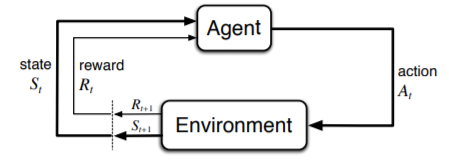
\includegraphics[width=0.8\columnwidth]{rl_diagram.png}
\caption{\label{fig:rl_diagram}Interaction between an agent and the environment it exists in \cite{r.s.sutton}.}
\end{figure}

\subsubsection{Q-Learning}
Q-Learning involves learning an action-value function, $Q(S, A)$, which maps states and actions to a value $Q$. To learn the action-value function, an iterative update is used as shown in equation \ref{eq:q_update}

\begin{equation}
	\label{eq:q_update}
	Q(s_t, a_t) = (1-\alpha_t) Q(s_t, a_t) + \alpha_t [R_{t+1} + \gamma max_a Q(s_{t+1}, a_{t+1})]
\end{equation}

At each time step the Q-value for the previous state-action pair, $s_t$ and $a_t$, is updated at a learning rate, $\alpha_t$, by the sum of the received reward, $R_t$, and the discounted Q-value of the next state, $s_{t+1}$, maximized by selecting action $a_{t+1}$. The simplest way to represent the action-value function is to tabulate the values, with each row representing a possible state, and each column representing a possible action. By initializing the table randomly and then letting the agent act according to its policy, $\pi$, the agent can learn the Q-values for each element of the table.

A simple policy that can be used for Q-Learning is the $\epsilon$-greedy policy. With this policy, the agent will either take the action that maximizes its current action-value function, $Q_t$, given its current state, or take a random action from the set of possible actions. The possibility that the agent takes a random action is determined by a the value $\epsilon$, where $0<\epsilon<1$. A higher value of $\epsilon$ means the agent explores more, while a lower value of $\epsilon$ means the agent exploits its current knowledge more. If $\epsilon=0$ the agent will always try to maximize its current action-value function and will not try new actions, which could potentially result in higher rewards. If $\epsilon=1$ the agent will always act randomly, which is useless in most cases. There is always a trade-off between exploitation and exploration, but certain tricks can be used to maximize reward, such as decreasing the exploration rate, $\epsilon$, as time passes and the agent learns to take optimal actions.

\subsubsection{Function Approximation}
Although tabulated Q-Learning is simple, many problems cannot be described in a discrete way. Function approximation provides a way to model the action-values in a continuous state space using a learned function. Most commonly, the Q function is represented by a neural network that takes the state as its input, and outputs a vector of the action-values for each action in the discrete action space. The update function shown in equation \ref{eq:func_approx} is similar to the tabular case, but uses the difference between the current Q-value and the next reward plus the next Q-value as the error term in the backpropagation for the neural network.

\begin{equation}
\begin{split}
	\label{eq:func_approx}
	& E = [R_{t+1} + \gamma max_a Q(s_{t+1}, a_{t+1})] - Q(s_t,a_t) \\
	& w_{i,j} \leftarrow w_{i,j} + \alpha_t \frac{\di E}{\di w_{i,j}}
\end{split}
\end{equation}


\section{Proposed Solutions}
\subsection{Criteria and Constraints}

The proposed solutions for the project were constrained according to the following constraints.
\begin{itemize}
		\item The solution must improve the performance of the automatic levelling wrist.
    \item The solution must implement machine learning in some way.

\end{itemize}

The following criteria considered in choosing an appropriate solution are chosen such that the automatic levelling wrist reliably improves the user's ability to use the prosthetic.
\begin{itemize}
    \item The solution should minimize steady state error.
		\item The solution should minimize response time.
		\item The solution should minimize settling time.
		\item The solution should maximize reliability and consistency.
\end{itemize}
Due to the nature of the problem, training time and data are difficult to acquire. Without a simulation, data and training can only be collected and run in real time. Therefore, the solution should require minimal training time and data, or be able to make use of a simulation.

\subsection{Neural Network Methods}
The three neural network methods proposed in this section make use of the PID control loop described in Figure \ref{fig:servo_system}. A neural network that outputs the PID gains, $K_p$, $K_i$, and $K_d$ is added to the control loop. The idea is that the neural network will learn to output appropriate gains for any situation, such that the system has the best response time and error for that situation. The rotation and flexion servos will use separately trained neural networks to output gains for their respective PID controllers. In this section the rotation servo will be used to explain the method, but the same method can be applied to both rotation and flexion servos.
\subsubsection{PID Auto-Tuning, Trained Model-Free using Backpropagation}\label{sec:model_free_backprop}
Since no labels exist for the PID gains at the output of the neural network (it is unknown what the gains should be in any given situation) the error term used to train the neural network, $E$, must be the squared error between the servo angle, $\phi(t)$ and the setpoint, $r(t)$ as shown in equation \ref{eq:model_free_error}. To train the neural network, this error must be backpropagated through the servo and the PID controller to the neural network output, $\bf{m}$. Performing the chain rule on the partial derivative of $E$ with respect to $\bf{m}$ yields \ref{eq:backprop_servo}. This partial derivative can then be backpropagated through the neural network to train the weights.

\begin{equation}
	\label{eq:model_free_error}
	E = \frac{1}{2}(r - \phi)^2
\end{equation}

\begin{equation}
	\label{eq:backprop_servo}
	\frac{\di E}{\di \bf{m}} =
	\begin{bmatrix}
		\frac{\di E}{\di \phi} \frac{\di \phi}{\di u} \frac{\di u}{\di K_p} \\
		\frac{\di E}{\di\phi} \frac{\di \phi}{\di u} \frac{\di u}{\di K_i} \\
		\frac{\di E}{\di \phi} \frac{\di \phi}{\di u} \frac{\di u}{\di K_d}
	\end{bmatrix}
\end{equation}

Here, $phi$ is the rotation servo angle, $u$ is the control signal from the PID controller defined in equation \ref{eq:pid}, and $K_p$, $K_i$, and $K_d$ are the PID gains. The solutions to the individual partial derivatives are shown in equation \ref{eq:partial_derivs}

\begin{equation}
\begin{split}
	\label{eq:partial_derivs}
	& \frac{\di E}{\di \phi} = r - \phi \\
	& \frac{\di \phi}{\di u} = ? \\
	& \frac{\di u}{\di K_p} = e(t) \\
	& \frac{\di u}{\di K_i} = \int e(t)dt \\
	& \frac{\di u}{\di K_d} = \frac{de(t)}{dt} \\
\end{split}
\end{equation}

Since the time domain function of the servo, $\phi(t)$ is not known, it is not possible to solve for $\frac{\di \phi}{\di u}$. To address this problem, a second neural network that mimics the servo can be used in the backpropagation rather than the actual servo. This allows the error to be backpropagated through the neural network, through the PID controller and to the PID neural network. Figure \ref{fig:pid_model_free_backprop} is the control loop block diagram with the added PID neural network and servo neural network. The servo neural network will be trained on the actual response of the servo. By treating the input to the servo as the input to the neural network, and the output of the servo as the labels for training, backpropagation can be performed to train the servo neural network on dataset of inputs and outputs given by the actual servo. Once trained, the neural network can be implemented into the control loop to train the PID neural network.

\subsubsection{PID Auto-Tuning, Trained Model-Free using the Levenberg-Marquardt Algorithm}
Rather than using backpropagation to train the weights of the PID neural network, the Levenberg-Marquardt algorithm is used to train the PID neural network as described in section \ref{sec:levenberg}. Equation \ref{eq:levenberg_model_free} is used to solve for the weight adjustments, $\sigma$, using the difference between the servo angle, $\phi$, and the setpoint, $r$, as the error term. A servo neural network, trained the same way as described in sec\ref{sec:model_free_backprop} is used to simulate the servo response to small weight changes needed to calculate the jacobian of the servo outlined in section \ref{sec:numerical_jacobian}.

\begin{equation}
	\label{eq:levenberg_model_free}
	\sigma = [J_w^T J_w + \lambda I]^-1 J_w^T [\phi - r]
\end{equation}

\subsubsection{PID Auto-Tuning, Trained with a Model using the Levenberg-Marquardt Algorithm}


PID auto-tuning trained model-free, using backpropagation
PID auto-tuning trained model-free, using the Levenberg-Marquardt algorithm
PID auto-tuning trained with a model, using the Levenberg-Marquardt algorithm


\subsection{Reinforcement Learning Methods}
Tabular Q-learning
Q-learning with function approximation


\section{Solution Evaluation}
\subsection{Q-learning - Tabular}
Tabular control wasn't granular enough to enable precise control of the servo
Even with a minimized state space (only using the IMU angle), it was still difficult to visit all states and learn making it unreliable.
\subsection{Q-learning - Function Approximation}
Not enough data to train the neural network, difficult to visit all states, no simulation (must train real-time which is very slow especially if testing different hyperparameters)
Deadly triad (bootstrapping, function approximation and off-policy learning) - not guaranteed to converge

\subsection{PID Auto-Tuning - Trained with Model, using Levenberg-Marquardt}
Requires a simulation for the servo, however the level of sophistication for the simulation does not need to be extremely high as in an RL setting. Uses a PID controller (so not starting from scratch) which makes it more reliable, as the PID controller on its own will achieve the objective of automatic levelling to a certain level. Therefore a simple simulation can be a starting point.
Quick training for the neural network, as a simulation can tune the neural network many times faster than real time.
\subsection{PID Auto-Tuning - Trained Model-Free, using Levenberg-Marquardt}
Quick training for the neural network, as a simulation can tune the neural network many times faster than real time. However, another neural network must be trained to emulate the real system which requires real data. It was found that there was not enough real data to generalize to all situations. (generalizes well to what it saw, but not anything else like the APRBS used to find the jacobian)
\subsection{PID Auto-Tuning - Trained Model-Free, using backpropagation}
Same problems as above, as well as being difficult to implement, due to the statefulness of the PID controller.

\subsection{Chosen Solution}
The chosen solution was PID auto-tuning trained using a model, using the Levenberg-Marquardt algorithm.

\section{PID Auto-Tuning Implementation}
Required components: a transfer function or ode for the servo, a simulation, a neural network, a numerical implementation of the levenberg marquardt algorithm, a numerical jacobian calculator, an APRBS generator, a neural network implemented in C\#
\subsection{Servo Transfer Function}

\subsection{Single DOF Simulation}
Best parameters for simulation

\subsection{Neural Network Structure}
5 inputs (error, angle, velocity), 4 nodes in hidden layer, 3 output nodes, leaky relu with alpha=0.3 activation function. Absolute value of output to keep positive (can't have negative gains)

\subsection{Levenberg-Marquardt Algorithm Implementation}


\subsection{Amplitude Modulated Pseudo-Random Binary Signal (APRBS) Generation}



\begin{table}[H]
	\begin{center}
		\caption{Sample table2}
        \label{tab:sampletable}
        \begin{tabular}{l|l|l|l|l}
        Requests/Second & Required Size & Cores & Memory (GiB) & Cost (\$/month)\\
        \hline
        10 & t2.small & 1 & 2 & 16.56\\
        100 & t2.medium & 2 & 4 & 33.41\\
        1000 & t2.large & 2 & 8 & 66.82\\
        10000 & t2.xlarge & 4 & 16 & 133.63\\
        \end{tabular}
	\end{center}
\end{table}

\begin{equation}
\label{eq:equation}
Sample equation
\end{equation}

\begin{figure}[H]
\centering 
\includegraphics[width=0.8\columnwidth]{UW.jpg}
\caption{\label{fig:figure}Sample figure}
\end{figure}
\pagebreak

\section{Results}

\section{Conclusion}

\section{Recommendations}
Better Simulation (2 DOF, better approximation of moment of inertia for different servo positions, take torque due to gravity into account)


\pagebreak

\begin{thebibliography}{99}
\bibitem{n.m.bajaj}
N. M. Bajaj, A. J. Spiers, and A. M. Dollar, “State of the art in prosthetic wrists: Commercial and research devices”, in \textit{2015 IEEE International Conference on Rehabilitation Robotics
(ICORR)}, Aug. 2015, pp. 331–338.

\bibitem{s.l.carey}
S. L. Carey, M. J. Highsmith, M. E. Maitland, and R. V. Dubey, “Compensatory movements
of transradial prosthesis users during common tasks”, \textit{Clinical Biomechanics}, vol. 23, no. 9,
pp. 1128 –1135, 2008.



\bibitem{k.ostlie}
K. Østlie, R. J. Franklin, O. H. Skjeldal, A. Skrondal, and P. Magnus, “Musculoskeletal pain
and overuse syndromes in adult acquired major upper-limb amputees”, \textit{Archives of Physical
Medicine and Rehabilitation}, vol. 92, no. 12, pp. 1967 –1973, 2011.

\bibitem{d.j.a.brenneis}
D. J. A. Brenneis, "Automatic Levelling of a Prosthetic Wrist", \textit{University of Alberta}, 2019.

\bibitem{r.s.sutton}
R. S. Sutton and A. G. Barto, "Introduction to reinforcement learning", \textit{Cambridge: MIT
Press}, second edition, 2018.
% \bibitem{whatisacodec}
% "What is a CODEC? And why is it an important component of videoconferencing?", \textit{Jwhornvideoconference.com}, 2018. [Online]. Available: http://www.jwhornvideoconference.com/what-is-a-codec-and-why-is-it-an-important-component-of-videoconferencing. [Accessed: 16- Aug- 2018].
%
% \bibitem{s3}
% "Cloud Object Storage", \textit{Amazon Web Services, Inc.}, 2018. [Online]. Available: https://aws.amazon.com/s3/. [Accessed: 16- Aug- 2018].
%
% \bibitem{ec2}
% "Amazon EC2", \textit{Amazon Web Services, Inc.}, 2018. [Online]. Available: https://aws.amazon.com/ec2. [Accessed: 16- Aug- 2018].
%
% \bibitem{lambda}
% "AWS Lambda – Serverless Compute", \textit{Amazon Web Services, Inc.}, 2018. [Online]. Available: https://aws.amazon.com/lambda/. [Accessed: 16- Aug- 2018].
%
% \bibitem{dynamodb}
% "Amazon DynamoDB", \textit{Amazon Web Services, Inc.}, 2018. [Online]. Available: https://aws.amazon.com/dynamodb/. [Accessed: 16- Aug- 2018].
%
% \bibitem{firewall}
% "What is firewall? - Definition from WhatIs.com", \textit{SearchSecurity}, 2018. [Online]. Available: https://searchsecurity.techtarget.com/definition/firewall. [Accessed: 16- Aug- 2018].
%
% \bibitem{querystring}
% "What is a Query String?", \textit{Techopedia.com}, 2018. [Online]. Available: https://www.techopedia.com/definition/1228/query-string. [Accessed: 16- Aug- 2018].
%
% \bibitem{uuiddef}
% P. Leach, M. Mealling and R. Salz, "RFC 4122 - A Universally Unique IDentifier (UUID) URN Namespace", \textit{Tools.ietf.org}, 2005. [Online]. Available: https://tools.ietf.org/html/rfc4122\#section-4.2. [Accessed: 16- Aug- 2018].
%
% \bibitem{uuidunique}
% "Are UUIDs really unique?", \textit{Towards Data Science}, 2018. [Online]. Available: https://towardsdatascience.com/are-uuids-really-unique-57eb80fc2a87. [Accessed: 16- Aug- 2018].
%
% \bibitem{uuidunique2}
% "Advanced", \textit{2database.com}, 2018. [Online]. Available: http://www.h2database.com/html/advanced.html\#uuid. [Accessed: 16- Aug- 2018].
%
% \bibitem{statuscode}
% "HTTP/1.1: Status Code Definitions", \textit{W3.org}, 2018. [Online]. Available: https://www.w3.org/Protocols/rfc2616/rfc2616-sec10.html. [Accessed: 16- Aug- 2018].
%
% \bibitem{mvc}
% "MVC Framework Introduction", \textit{www.tutorialspoint.com}, 2018. [Online]. Available: https://www.tutorialspoint.com/mvc\_framework/mvc\_framework\_introduction.htm. [Accessed: 16- Aug- 2018].
%
% \bibitem{https}
% "What is HTTPS?", \textit{Techopedia.com}, 2018. [Online]. Available: https://www.techopedia.com/definition/5361/hypertext-transport-protocol-secure-https. [Accessed: 16- Aug- 2018].
%
%

\end{thebibliography}

\begin{appendices}
\section{Appendix}
\end{appendices}


\end{document}
